\documentclass{article}

\usepackage{graphicx}
\usepackage{tikz}
\usepackage{tikzsymbols}
\usetikzlibrary{calc,patterns,shapes.geometric}
\pagestyle{empty}
\usepackage[margin=0pt]{geometry}
\geometry{papersize={14in,12in}}

\def\centerarc[#1](#2)(#3:#4:#5){\draw[#1] ($(#2)+({#5*cos(#3)},{#5*sin(#3)})$) arc (#3:#4:#5);}

\begin{document}
	\begin{figure}
		\centering
		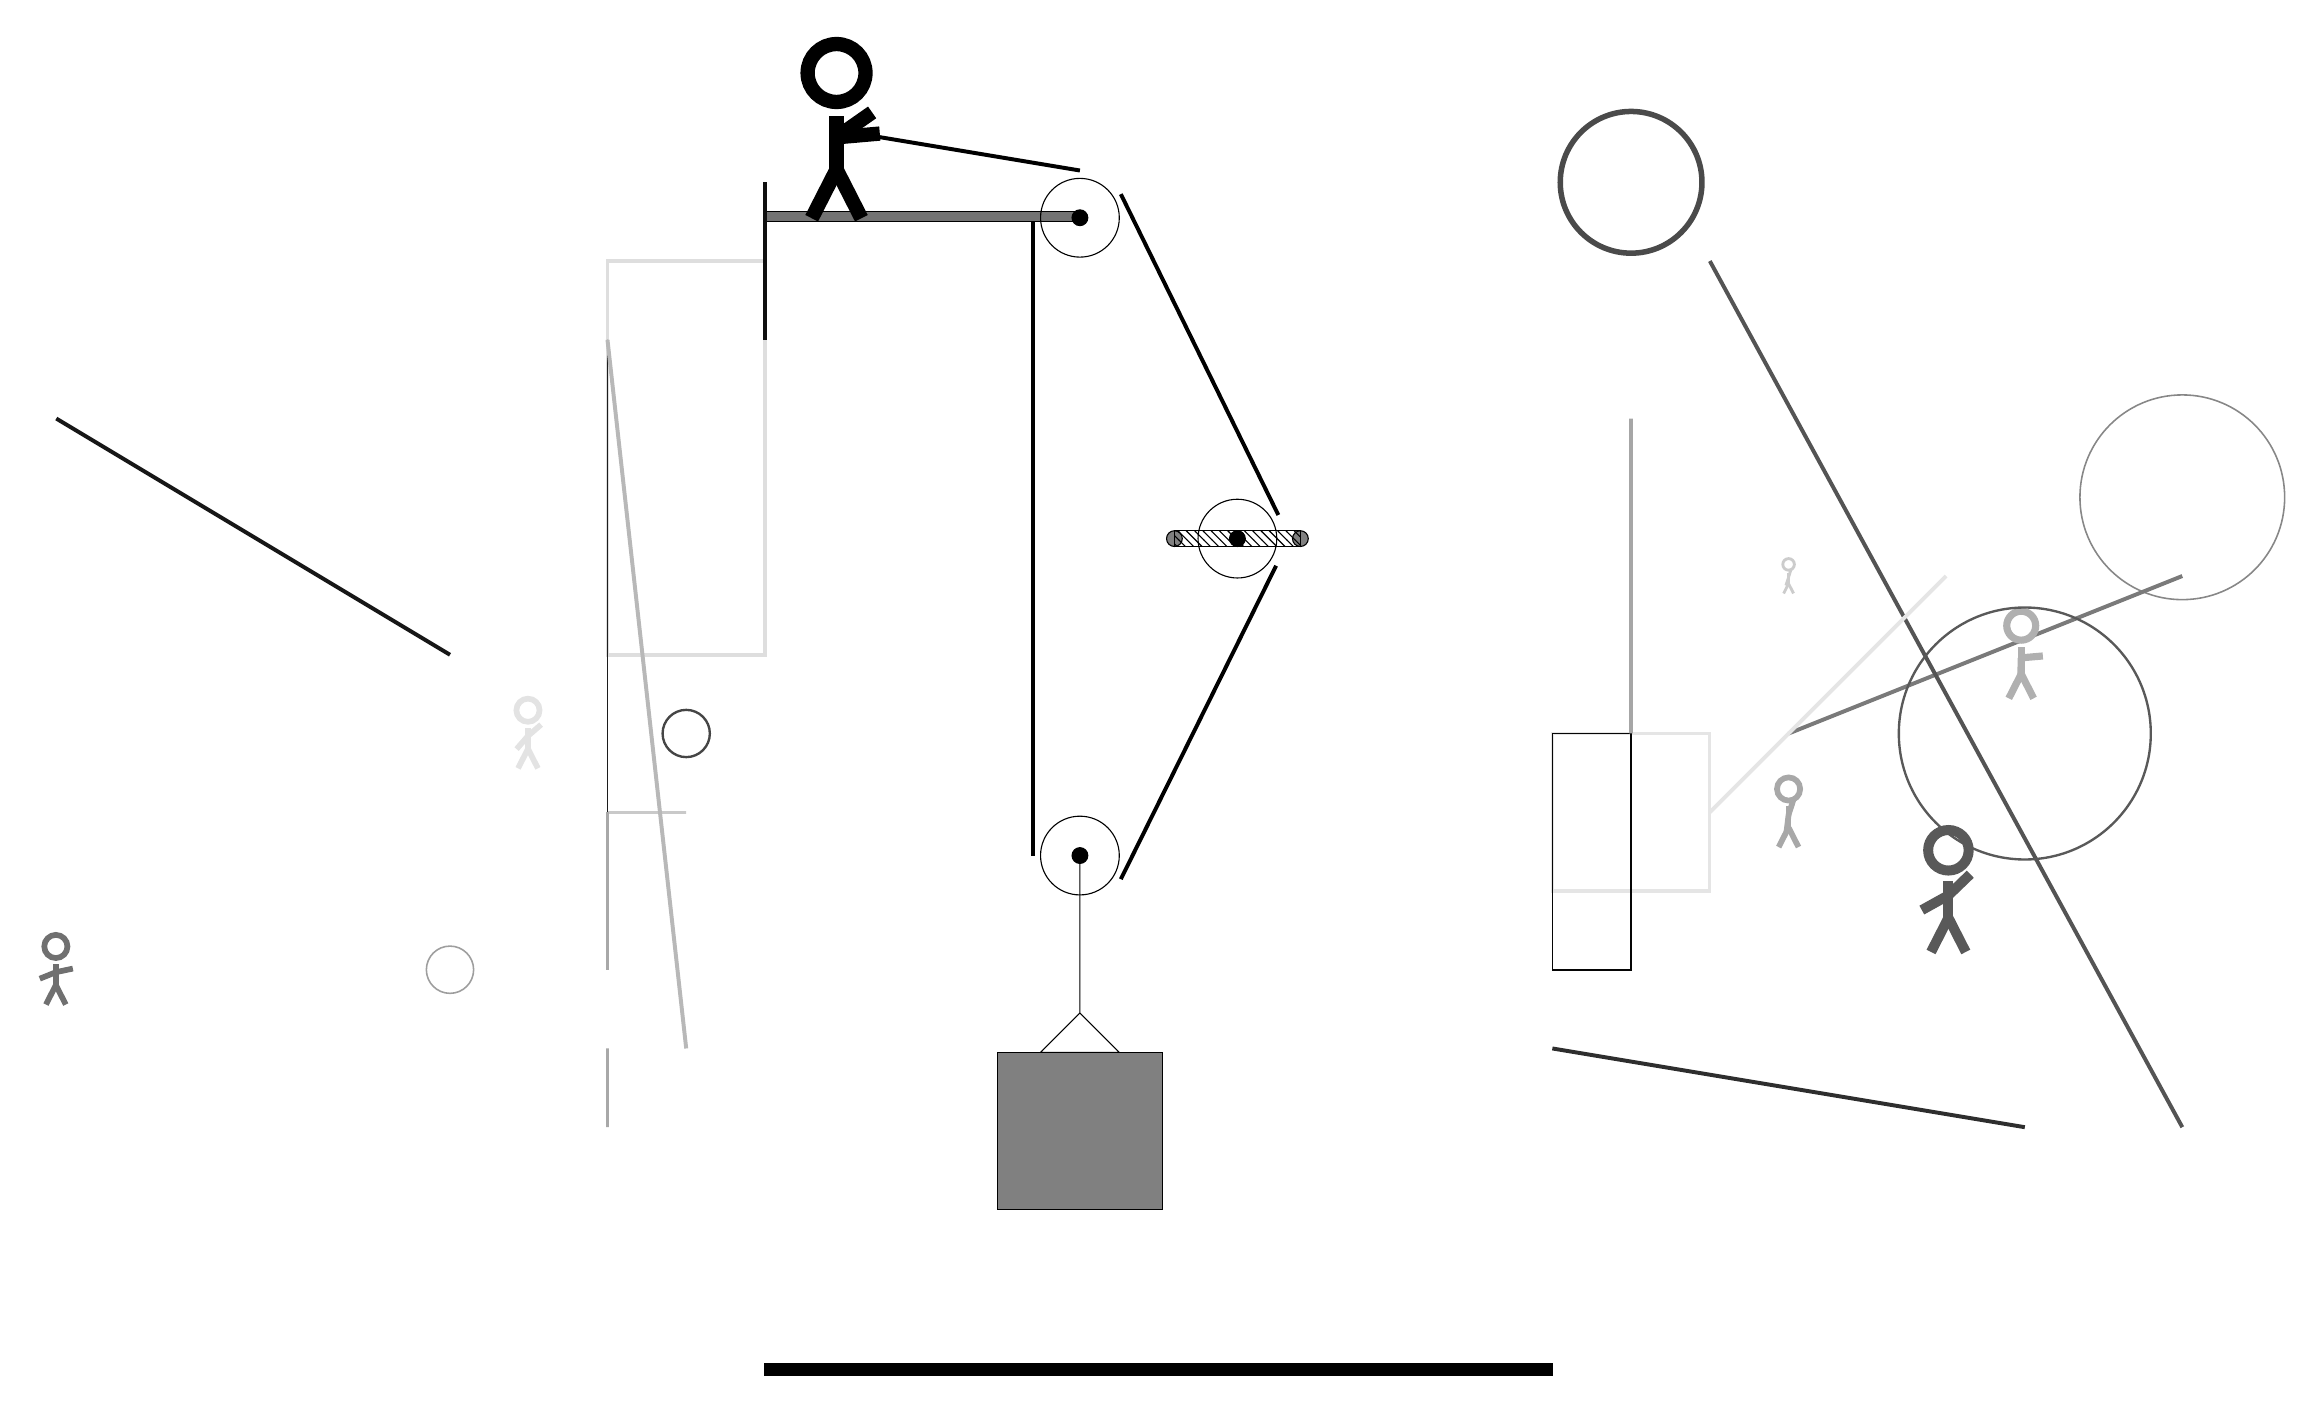
\begin{tikzpicture}
			%%%%% START %%%%%
			
			\draw[fill=black!55] (-2, 11.5) rectangle (2, 11.625);
			
			\draw (2, 3.45) circle (0.5);
			\draw[fill=black] (2, 3.45) circle (0.1);
			
			\draw (2, 11.55) circle (0.5);
			\draw[fill=black] (2, 11.55) circle (0.1);
			
			\draw[fill=white](4, 7.475) circle (0.5);
			\draw[fill=black] (4, 7.475) circle (0.1);
			\draw[fill=black!50] (3.2, 7.475) circle (0.1);
			\draw[fill=black!50] (4.8, 7.475) circle (0.1);
			\draw[pattern=north west lines, pattern color=black] (3.2, 7.575) rectangle (4.8, 7.375);
			
			\draw[line width=0.4mm, color=black!21] (-4, 4) rectangle (-3, 4);
			
			\draw[line width=0.5mm, color=black!13] (-2, 11) rectangle (-4, 6);
			\draw[line width=0.5mm, color=black!82](8, 1) -- (14, 0);
			\draw [line width=0.2mm, color=black!47](16, 8) circle (1.3);
			
			\node[line width=0.7mm, color=black!11] at (-5, 5) {\Strichmaxerl[4][49][41]};
			\draw[line width=0.5mm, color=black!52](11, 5) -- (16, 7);
			\draw[line width=0.2mm, color=black!89] (-4, 2) rectangle (-4, 10);
			\draw[line width=0.5mm, color=black!28](-4, 10) -- (-3, 1);
			\draw[line width=0.5mm, color=black!34](-4, 2) -- (-4, 4);
			\draw[line width=0.4mm, color=black!10] (10, 3) rectangle (8, 5);
			
			\draw[line width=0.4mm, color=black!34] (-4, 1) rectangle (-4, 0);
			
			\draw [line width=0.2mm, color=black!38](-6, 2) circle (0.3);
			\draw[line width=0.5mm, color=black!67](10, 11) -- (16, 0);
			
			\node[line width=0.4mm, color=black!20] at (11, 7) {\Strichmaxerl[2][72][73]};
			\node[line width=0.4mm, color=black!65] at (13, 3) {\Strichmaxerl[7][29][44]};
			\node[line width=0.5mm, color=black!31] at (14, 6) {\Strichmaxerl[5][89][5]};
			
			\node[line width=0.6mm, color=black!34] at (11, 4) {\Strichmaxerl[4][83][72]};
			
			\draw[line width=0.5mm, color=black!10](13, 7) -- (10, 4);
			\draw[line width=0.2mm, color=black!98] (8, 2) rectangle (9, 5);
			\draw [line width=0.3mm, color=black!65](14, 5) circle (1.6);
			\node[line width=0.3mm, color=black!56] at (-11, 2) {\Strichmaxerl[4][22][12]};
			
			\draw[line width=0.5mm, color=black!94](-2, 12) -- (-2, 10);
			
			\draw[line width=0.5mm, color=black!91](-6, 6) -- (-11, 9);
			\draw [line width=0.7mm, color=black!71](9, 12) circle (0.9);
			\draw [line width=0.3mm, color=black!73](-3, 5) circle (0.3);
			
			\draw[line width=0.6mm, color=black!35] (9, 5) rectangle (9, 9);
			
			
			\draw (2, 3.45) -- (2, 1.45) -- (1.5, 0.95) -- (2.5, 0.95) -- (2, 1.45);
			\draw[fill=black!50] (0.95, 0.95) rectangle (3.05, -1.05);
			
			\draw[line width=0.5mm] (1.4, 11.5) -- (1.4, 3.45);
			\centerarc[line width=0.5mm](2, 3.45)(180:330:0.6);
			\draw[line width=0.5mm](2.5196, 3.15) -- (4.4915, 7.1308);
			\centerarc[line width=0.5mm](4, 7.475)(390:325:0.6);
			\draw[line width=0.5mm](4.5196, 7.775) -- (2.5196, 11.85);
			\centerarc[line width=0.5mm](2, 11.55)(30:90:0.6);
			\draw[line width=0.5mm](2, 12.15) -- (-1, 12.65);
			
			\node at (-1, 12.65) {\Strichmaxerl[10][-175][35]};
			
			\draw[fill=black] (-2, -3) rectangle (8, -3.15);
			
			%%%%% END %%%%%
		\end{tikzpicture}
	\end{figure}	
\end{document}